\chapter{Results, Analysis, and Evaluation}

\section{Software Testing}

\subsection{Backend Testing}

The \textit{ASACBackEnd} project adopts a strong testing plan to ensure the reliability of each component within its application. The tests are based on \texttt{Django's testing framework}, with extra help from \texttt{Pytest}. Every application of the \textit{ASACBackEnd} project, whether \textit{Forums}, \textit{Contracts}, \textit{Accounts}, or \textit{Notifications}, includes a directory called \textit{``tests''} containing test files corresponding to each module written. To make tests predictable and separate them from outside services, such as sending notifications or interacting with the AI model, \textit{unittest.mock} library is utilised.

The \texttt{pytest.ini} configuration file sets up the testing environment through the following flags:

\begin{itemize}
    \item \textbf{``DJANGO\_SETTINGS\_MODULE''}: Set to \textit{ASACBackEnd.settings} for correct context during test runs.
    \item \textbf{``asyncio\_mode''}: Set to \textit{auto} to enable asynchronous input and output operations.
    \item \textbf{``addopts''}: Includes options like \textit{``--nomigrations''} to disable migrations for faster test execution, \textit{``--cov=.''} for enabling coverage measurements, and \textit{``-cov-report=term-missing''} for terminal coverage reports.
    \item \textbf{``python\_files''}: Specifies test file recognition patterns: their names are either \textit{``tests.py''}, they start with \textit{``test\_*''}, or end with \textit{``*\_tests.py''}. 
    \item \textbf{``testpaths''}: Specifies directories for \textit{pytest} to find test files.
    \item \textbf{``norecursedirs''}: Lists directories to ignore during test search, including hidden directories, \textit{venv}, \textit{sdist}, \textit{build}, \textit{node modules}, and \textit{Django} migration files.
    \item \textbf{``.coveragerc''}: Configures coverage reporting.
\end{itemize}

\subsubsection{Testing ASGI and WSGI Configurations}

Tests for synchronous and asynchronous requests are found in \textit{test\_wsgi.py} and \textit{test\_asgi.py} files. These tests ensure proper configuration of \textit{WSGI} and \textit{ASGI} applications to handle WebSocket and HTTP traffic. The middleware stack and routing protocols are also verified.

\subsubsection{Testing Settings}

In \textit{test\_settings.py}, the configuration tests confirm that database settings, middleware, and installed apps are applied correctly for different environments (development, testing, production). Additionally, authentication methods and CORS headers are also checked for security purposes. 

\subsubsection{Testing Admin Interfaces}

Admin tests, as shown in each testing subdirectory of every application within the \textit{test\_admin.py} files, verify that models are correctly registered with Django's admin. Alongside, they also check if admin pages render accurately (this includes list and detail views). This testing often involves using \textit{RequestFactory} to simulate admin interface requests.

\subsubsection{Testing Application Configuration}

Application configuration tests, located in files named \textit{test\_apps.py}, verify that Django applications are correctly initialised.

\subsubsection{Testing Models}

In each \textit{``tests''} subdirectory of each application, there is a file named \textit{test\_models.py}. These files typically contain test cases that validate the business logic embedded in the models, relationships, and custom methods. The Django \textit{TestCase} class is used extensively for database interaction, utilising Django's database rollback functionalities to ensure test isolation.

Model testing involves:
\begin{itemize}
    \item Validating model fields and attributes.
    \item Checking model methods for expected behavior.
    \item Ensuring the integrity of relationships between models.
\end{itemize}

\subsubsection{Testing Serialisers}

Serialisers are tested to ensure that they accurately serialise and deserialise data. These tests, located in each subdirectory of each application under \texttt{test\_serialisers.py}, check:
\begin{itemize}
    \item Field validation.
    \item Output data structure.
    \item Integration with models for creating and updating records.
\end{itemize}

\subsubsection{Testing URL Routing}

Routing tests in each subdirectory of each application in files named \textit{test\_urls.py} verify that URLs correctly map to views. The tests utilise Django's \textit{resolve} and \textit{reverse} functions to simulate web requests and ensure endpoints are accessible.

\subsubsection{Testing Validators}

In the \textit{test\_validators.py} file, tests ensure that custom validation logic in models or serialisers behaves as expected. These tests:

\begin{itemize}
    \item Validate input data for compliance with defined rules, ensuring data integrity.
    \item Use Python's built-in \texttt{ValidationError} to ensure that invalid data is caught and handled properly.
\end{itemize}

\subsubsection{Testing Views}

View tests in \textit{test\_views.py} files ensure HTTP interfaces function as expected, checking response status codes, data structure, and handling of authentication and permissions. Mocking is extensively used to isolate view tests from external dependencies.

\subsubsection{Testing Consumers}

Testing \textit{WebSocket} consumers, as outlined in \texttt{test\_consumers.py}, includes:

\begin{itemize}
    \item Using the \texttt{WebsocketCommunicator} to simulate web socket interactions, testing both the connection lifecycle and message handling.
    \item Ensuring that messages sent over web sockets are received and broadcast correctly to all connected clients, using Django Channels' groups and messaging layers.
\end{itemize}

\subsubsection{Testing Routing}

Routing tests for web sockets ensure that the \texttt{WebSocket} URLs are correctly configured to handle incoming connections, as shown in \texttt{test\_routing.py}.

\subsubsection{Testing Utility Functions}

Utility function tests in \textit{test\_utils.py} focus on external integrations and side effects such as sending notifications. These tests:

\begin{itemize}
    \item Often use mocking to simulate external services and verify that utilities behave correctly under different scenarios without sending actual requests.
    \item Check that the functions handle errors correctly and perform their intended side effects.
\end{itemize}

\subsubsection{Coverage}

Comprehensive testing is one of the most important aspects of maintaining software reliability. Hence, by achieving a 100\% coverage combined with continuous integration, the backend achieves stability and dependability.

\begin{figure}[!ht]
    \centering
    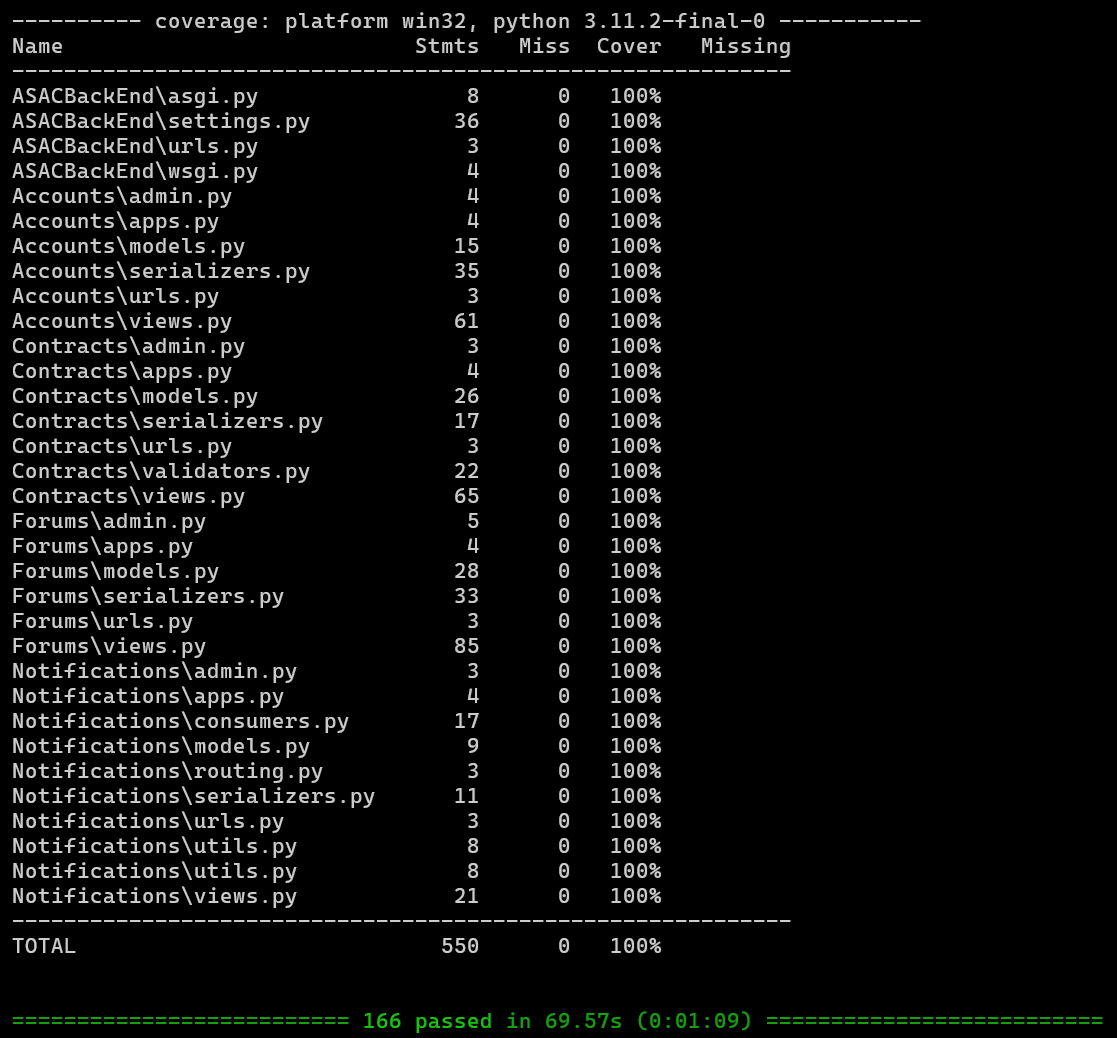
\includegraphics[width=1\textwidth]
    {LATEX/Appendices/Images/Software/Backend/backend_testing_report.png}
    \caption{Backend Test Coverage Report}
    \label{fig:backend_testing}
\end{figure}

\subsection{Frontend Testing}

The \texttt{\_\_tests\_\_} folder in the root directory of the UI contains the test files for the application. Each test file is stored in a structure that mirrors the corresponding file in the root directory and is named similarly but with \texttt{.test.js} at the end. The configuration for testing is set up as follows in the \texttt{package.json} file:

\begin{itemize}
    \item \textbf{Jest Configuration}: For compatibility with Expo, \textit{``preset''} is set to \textit{jest-expo}. \textit{JavaScript} and \textit{TypeScript} files are transformed using \textit{babel-jest} specified under the \textit{``transform''} parameter. Coverage data is gathered from designated files specified in \textit{``collectCoverageFrom''} and is enabled with \textit{``collectCoverage''}. The output format of coverage reports is defined in \textit{``coverageReporters''}, and strict coverage thresholds are set through \textit{``coverageThreshold''} to 100\% for branches, functions, lines, and statements. Module handling is managed by \textit{``moduleFileExtensions''} for file extensions, \textit{transformIgnorePatterns''} for excluding modules during transformation, and \textit{``setupFilesAfterEnv''} configures \textit{@testing-library/jest-native/extend-expect} for post-environment setup.
\end{itemize}

\paragraph{Additional Information}

This section summarises the recurring elements used across all test suites. To avoid redundancy, these details will not be reiterated in the future.

\begin{itemize}
    \item \textbf{Setup Configuration:} Tests use Jest and the React Native Testing Library.
    \item \textbf{Imports and Mock Implementations:}
    \begin{itemize}
        \item Essential imports typically include \textit{React}, \textit{react-native}, \textit{@react-navigation/native}, and \textit{render} from \textit{@testing-library/react-native}.
        \item Each test file has its own set of customised mocks, which usually cover modules such as \textit{expo-notifications}, \textit{@react-navigation}, \textit{expo-file-system}, \textit{AppNavigator}, \textit{ErrorBoundary}, \textit{Authentication}, \textit{Keyboard}, \textit{Theme}, and custom hooks used to control the screens.
    \end{itemize}
    \item \textbf{Test Suites:}
    \begin{itemize}
        \item Are defined with \texttt{describe(``<Name of the original application>'', ...)} and contain multiple test cases.
        \item \texttt{beforeEach} and \texttt{afterEach} blocks are used to set up and then clear mocks to achieve a clean environment for each test.
    \end{itemize}
    \item \textbf{General Tests Execution:}
    \begin{itemize}
        \item \textbf{Environment:} Each component is tested within its respective provider environment to simulate real application conditions.
        \item \textbf{Methodology:} Makes considerable use of assertions to confirm anticipated results while simulating external dependencies with the help of mocks, ensuring test isolation.
        \item \textbf{Cleanup:} Ensures that mocks are cleared and functions restored post-testing to prevent test contamination.
    \end{itemize}
\end{itemize}

\subsubsection{Testing Root Directory}

\begin{itemize}
    \item \textbf{App.test.js:}
    \begin{itemize}
        \item These tests aim to confirm that the main application component properly integrates its submodules while managing notifications and global settings.
        \item The setup includes \textit{expo-notifications}, \textit{AppNavigator}, \textit{ErrorBoundary}, and other necessary modules.
        \item \textbf{Core Tests:}
        \begin{itemize}
            \item \textbf{Platform Specific Behaviour}: Checks whether \textit{Android} devices have layout animation turned on.
            \item \textbf{Error Handling}: Ensures that the global error handler is configured correctly in development mode and accurately logs errors.
            \item \textbf{Notification Management}: Tests handling of notifications, ensuring correct configuration and cleanup of notification listeners.
            \item \textbf{Component Rendering}: Verifies that the \textit{AppNavigator} is included as a child component in order to ensure that the app is rendering correctly.
        \end{itemize}
    \end{itemize}

    \item \textbf{babel.config.test.js:}
    \begin{itemize}
        \item The objective of this test suite is to verify the correct loading of Babel configurations based on different environment settings.
        \item There is a helper function that uses \textit{loadConfig(envSetting)} to simulate configuration loading.
        \item \textbf{Core Tests:}
        \begin{itemize}
            \item \textbf{Environment Configurations:} Checks configuration correctness for default, test, and production environments by verifying the appropriate inclusion of presets and plugins.
        \end{itemize}
    \end{itemize}

    \item \textbf{ErrorBoundary.test.js:}
    \begin{itemize}
        \item The goal of this test suite is to evaluate the \textit{ErrorBoundary's} capacity to catch and handle errors from child components.
        \item The setup utilises a \textit{ProblemChild} component that simulates error scenarios.
        \item \textbf{Core Tests:}
        \begin{itemize}
            \item \textbf{Error Catching}: Tests error catching from child components and verifies logging.
            \item \textbf{Fallback UI}: Checks the display of fallback UI upon error detection.
            \item \textbf{Normal Rendering}: Ensures normal rendering behaviour when no errors are present.
        \end{itemize}
    \end{itemize}
\end{itemize}

\subsubsection{Testing Components Directory}

\begin{itemize}
    \item \textbf{Common Patterns}: Each test involves using mocks for \textit{expo-secure-store}, \textit{global.fetch}, and \textit{WebSocket} to simulate external interactions.

    \item \textbf{Authentication.test.js:}
    \begin{itemize}
        \item \textbf{Objective:} Ensures authentication module works properly.
        \item \textbf{Setup and Mocks:} Uses mocks for \textit{expo-secure-store}, \textit{global.fetch}, and \textit{WebSocket} to simulate external interactions.
        \item \textbf{Core Tests:}
        \begin{itemize}
            \item \textbf{Token Validation:} Verifies that the token validation process correctly identifies valid and invalid tokens and handles network errors appropriately.
            \item \textbf{Sign Up:} Tests cover user registration scenarios, including missing fields, password mismatches, and server error responses.
            \item \textbf{Login and Logout Processes:} Tests check how tokens are managed and how errors are communicated to the user.
        \end{itemize}
    \end{itemize}

    \item \textbf{Keyboard.test.js:}
    \begin{itemize}
        \item \textbf{Objective:} Evaluates the \textit{KeyboardProvider's} ability to manage keyboard visibility during text input interactions.
        \item \textbf{Setup and Mocks:} Mocks \textit{Keyboard}, \textit{Dimensions}, and \textit{TextInput} to control keyboard and screen interactions.
        \item \textbf{Core Tests:}
        \begin{itemize}
            \item \textbf{Keyboard Visibility:} Ensures that keyboard visibility state updates correctly in response to show and hide events.
            \item \textbf{Reference Registration:} Tests the proper registration and unregistration of scroll view and text input references, assessing cleanup on component unmount.
            \item \textbf{Interaction with TextInput:} To make sure that input fields are not obscured by the keyboard, this test examines how the UI adjusts the view when a text input is focused.
        \end{itemize}
    \end{itemize}

    \item \textbf{Notifications.test.js:}
    \begin{itemize}
        \item \textbf{Objective:} Tests the reliability of \textit{WebSocket} connections and the scheduling of push notifications.
        \item \textbf{Setup and Mocks:} Involves mocking \textit{expo-secure-store}, \textit{expo-notifications}, \textit{global.fetch}, and \textit{WebSocket}.
        \item \textbf{Core Tests:}
        \begin{itemize}
            \item \textbf{WebSocket Management:} Verifies the correct opening and closing of web socket connections, including error handling.
            \item \textbf{Notification Handling:} Focuses on how incoming messages trigger notification scheduling and how token management operations handle errors.
            \item \textbf{Integration and Context Provision:} Checks for the maintenance of functional integrity by making sure that the web socket context is correctly provided to child components.
        \end{itemize}
    \end{itemize}

    \item \textbf{Theme.test.js:}
    \begin{itemize}
        \item \textbf{Objective:} Tests the theme management functionality.
        \item \textbf{Setup and Mocks:} Mocks \textit{expo-secure-store} for simulating theme storage operations.
        \item \textbf{Core Tests:}
        \begin{itemize}
            \item \textbf{Default Theme Settings:} Confirms that the default ``light'' theme is correctly set upon initialisation.
            \item \textbf{Theme Initialisation:} Checks the retrieval and setting of the theme from storage at startup.
            \item \textbf{Theme Toggling:} Verifies that the ``light'' and ``dark'' theme toggles are applied successfully and that the preferences are saved.
            \item \textbf{Dark Mode Detection:} Verifies that the application accurately detects the dark mode setting based on the stored theme preference.
        \end{itemize}
    \end{itemize}
\end{itemize}

\subsubsection{Testing Navigation Directory}

\begin{itemize}
    \item \textbf{AppNavigator.test.js:}
    \begin{itemize}
        \item Using mocked contexts for authentication and theme, tests verify that the \textit{AppNavigator} correctly renders navigation stacks based on the user's authentication status.
        \item \textbf{Core Tests:}
        \begin{itemize}
            \item Verification of \textit{PostLoginTabs} rendering when a user is authenticated.
            \item Verification of \textit{PreLoginStack} rendering when a user is unauthenticated.
        \end{itemize}
    \end{itemize}

    \item \textbf{PreLoginStack.test.js:}
    \begin{itemize}
        \item Concentrates on checking the correct rendering of screens within the \textit{PreLoginStack} through verifying the accessibility of all navigation screens for unauthenticated users via navigation simulations.
    \end{itemize}

    \item \textbf{PostLoginTabs.test.js:}
    \begin{itemize}
        \item Tests the \textit{PostLoginTabs} for correct rendering of tabs.
        \item \textbf{Core Tests:}
        \begin{itemize}
            \item Verification of tab functionality and correct rendering of associated stacks, including navigation simulations.
            \item Theme-specific rendering checks to ensure both light and dark modes are correctly applied.
        \end{itemize}
    \end{itemize}
    
    \item \textbf{Debugging and Resolution:}
    \begin{itemize}
        \item Initially, tests were failing because of issues related to the \textit{SafeAreaProvider} wrapping the entire navigation structure. The screen and all components below it were not rendering correctly, leading to empty debug outputs. After numerous failed attempts to troubleshoot, extensive research was conducted. It was found that mocking the \textit{SafeAreaContext} and its related hooks resolved the issue \cite{StackOverflowSafeAreaContextIssue2021, GithubSafeAreaContextIssue2019}.
        \item This emphasises how important it is to mock environmental components correctly in Jest, which can often be under-documented.
    \end{itemize}
\end{itemize}

\subsubsection{Testing Styles Directory}

All style sheets are subjected to unit testing under the \textit{``styles''} directory. The strategy involved rendering and asserting the styles for both light and dark themes. Objectively speaking, this was the simplest aspect of UI testing so far.

\begin{itemize}
    \item \textbf{ThemeStyles.test.js:} The file ensures that theme-related styles are applied correctly across the components below.
    \item \textbf{GloballySharedStyles.test.js:} Tests global styles that are used across the application.
    \item \textbf{LocallySharedStylesPreLoginScreens.test.js:} Tests styles for pre-login screens.
    \item \textbf{LocallySharedStylesHomeScreens.test.js:} Ensures styles for home screens are accurate.
    \item \textbf{LocallySharedStylesForumScreens.test.js:} Tests styles specific to forum screens.
    \item \textbf{LocallySharedStylesSupportScreens.test.js:} This test file ensures the accuracy of the styles for the support screen.
    \item \textbf{LocallySharedStylesSettingsScreens.test.js:} Verifies styles for the settings screen.
\end{itemize}

\subsubsection{Testing Screens Directory: UI Components}

So far, we have discussed the testing for the files that were varying in their purpose and implementation significantly from one another, requiring different testing approaches. Within the screens directory, we encounter two types of files: those defining UI components and hooks named \textit{use<filename>}. Although the logical implementation of these UI and hook files is similar, the specific testing needs differ according to the libraries used in each component and the elements that require assertion. Additionally, the handling of API responses differs between these files.

The general structure of these tests involves:

\begin{itemize}
    \item \textbf{Rendering the Component:} Each screen is rendered within a mocked navigation (\textit{NavigationContainer} from \textit{@react-navigation/native}) and theme context (\textit{ThemeContext.Provider}) to confirm it functions correctly.
    \item \textbf{Mocking Dependencies:} Mocking is applied to the required libraries, including \textit{@react-navigation/native}, \textit{@expo/vector-icons}, and other screen-specific dependencies.
    \item \textbf{Assertions:} Tests make sure that components are displayed as intended by looking for the presence of UI elements. For example, checking if the \textit{``Create Contract''} button is rendered correctly.
    \item \textbf{User Interactions:} Simulating user interactions such as button presses, text input changes, and form submissions to confirm the UI behaves as expected. These interactions are tested using the \textit{fireEvent} function from \textit{@testing-library/react-native}.
    \item \textbf{State Management:} Verifying the components' function calls and state modifications. For example, checking if the correct functions are called when a button is pressed or if the state changes appropriately. This involves mocking screen-specific hooks to provide a controlled manner of execution.
    \item \textbf{Handling Themes:} Confirming that elements appear as intended in both themes by comparing the colours of different UI elements.
    \item \textbf{Handling Modals and Alerts:} Testing whether modals and alerts are displayed correctly based on the components' states.
\end{itemize}

The UI components tested include:

\begin{itemize}
    \item \textbf{HomeScreen.test.js:} This file tests the home screen's functionality, including rendering the screen with the correct UI elements, handling user interactions like uploading files and creating contracts, and verifying state management and theme handling.
    \item \textbf{EditorScreen.test.js:} This file tests the editor screen, verifying the correct rendering of the code editor, handling of file loading, and theme management.
    \item \textbf{ForumScreen.test.js:} This file tests the forum screen, confirming that posts are rendered correctly, user interactions like liking, creating and deleting posts are handled, and the navigation to the \textit{CommentScreen} works.
    \item \textbf{CommentScreen.test.js:} This file tests the comment screen to make sure comments are loaded correctly and users can add new ones.
    \item \textbf{SupportScreen.test.js:} This file tests the support screen, verifying that the UI renders properly alongside the chat functionality, including sending messages and displaying assistant responses.
    \item \textbf{SettingsScreen.test.js:} This file tests the settings screen. This includes verifying that switches for dark mode and notifications work correctly alongside the logout button and the correct rendering of the UI.
\end{itemize}

\subsubsection{Testing Screens Directory: Hooks}

As for the management of state and side effects of the UI components, it is done by the custom hooks. These will have to be tested using \textit{React's} testing utilities, focusing on their behaviour and interactions with external dependencies.

\begin{itemize}
    \item \textbf{Setup and Teardown:} Resetting mocks with \textit{beforeEach} so that there is no previous state before new test executions. 
    \item \textbf{Rendering the Hook:} Return values and functions from hooks can be accessed in a controlled way using \textit{renderHook} from \textit{@testing-library/react-hooks}.
    \item \textbf{Mocking Dependencies:} The \textit{jest.mock} function is used to create mock implementations of dependencies. The libraries mocked in hooks test files are, amongst others, \textit{expo-document-picker}, \textit{expo-secure-store}, \textit{expo-file-system}, and \textit{expo-sharing}.
    \item \textbf{Assertions:} Testing hooks' behaviour by checking the returned values and the functions they call.
    \item \textbf{Handling Side Effects:} This includes testing how hooks behave during API calls, file operations, and their respective layout animations. This involves checking if the correct functions are called and if the state updates appropriately.
    \item \textbf{Error Handling:} This bit involves checking if hooks handle errors gracefully, such as when an API call fails or a file operation throws an error. To test these, failures are simulated, and the appropriate error messages / alerts are checked.
\end{itemize}

The hooks tested include:

\begin{itemize}
    \item \textbf{useHomeScreen.test.js}: This file tests the \textit{useHomeScreen} hook. Tests cover file selection, validation, contract uploads, error handling, and state updates.
    \item \textbf{useEditorScreen.test.js}: This file tests the \textit{useEditorScreen} hook. Tests cover loading file content, updating the theme, encoding special characters, and handling file reading errors.
    \item \textbf{useForumScreen.test.js}: This file tests the \textit{useForumScreen} hook. Tests cover post creation, liking, deleting posts, error handling, and state updates.
    \item \textbf{useCommentScreen.test.js}: This file tests the \textit{useCommentScreen} hook. Tests include fetching comments, adding comments, handling API errors, and updating the comment list.
    \item \textbf{useSettingsScreen.test.js}: This file tests the \textit{useSettingsScreen} hook. Tests cover checking the initial notifications setting, enabling and disabling notifications, and handling API interactions.
\end{itemize}

\subsubsection{Coverage}

Thorough testing is a key part of the stability of the frontend application. By running tests over all components using modern testing practices and techniques, coupled with continuous integration, the frontend becomes reliable. It has been tested with 100\% coverage for the most important metrics, which include statements, branches, functions, and lines.

\begin{figure}[!ht]
    \centering
    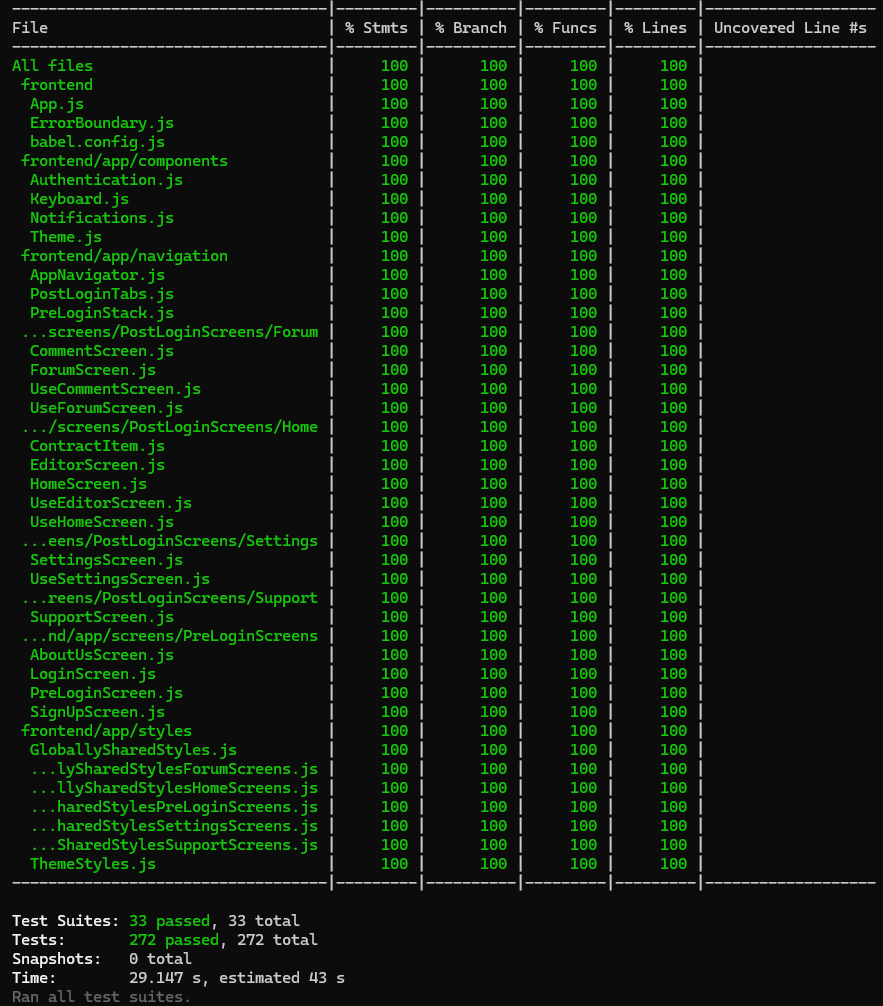
\includegraphics[width=1\textwidth]{LATEX/Appendices/Images/Software/Frontend/frontend_testing_report.png}
    \caption{Frontend Test Coverage Report}
    \label{fig:frontend_testing}
\end{figure}

\section{CI/CD Pipeline}

\subsection{Continuous Integration}

Through Continuous Integration, tests get automatically executed on a regular basis, which in turn improves software quality. The support for this feature was added for the backend and frontend codebases using \texttt{GitHub Actions}. The \texttt{CI/CD} pipeline is defined in the \textit{.github/workflows} directory, which is triggered anytime a push or pull request is made to the main branch. It is composed of several jobs, each responsible for a different part of the testing and deployment process, including:

\begin{itemize}
    \item The pipeline uses the \textit{actions/checkout@v2} action to checkout the repository code to the runner.
    \item Python 3.11.2 is set up using \textit{actions/setup-python@v2}.
    \item Node.js 18.14.0 is set up using \textit{actions/setup-node@v2}.
    \item The pipeline installs necessary Python dependencies from the \textit{requirements.txt} file.
    \item The pipeline installs necessary npm dependencies for the frontend. The installation process includes the \textit{legacy-peer-deps} flag to tackle compatibility issues.
    \item The code is linted using \textit{flake8} to ensure code quality. This step includes checking for errors, warnings, and generating a report.
    \item Backend tests are run using \textit{pytest}.
    \item Frontend tests are executed using the \textit{npm run test} command.
\end{itemize}

\begin{figure}[!ht]
    \centering
    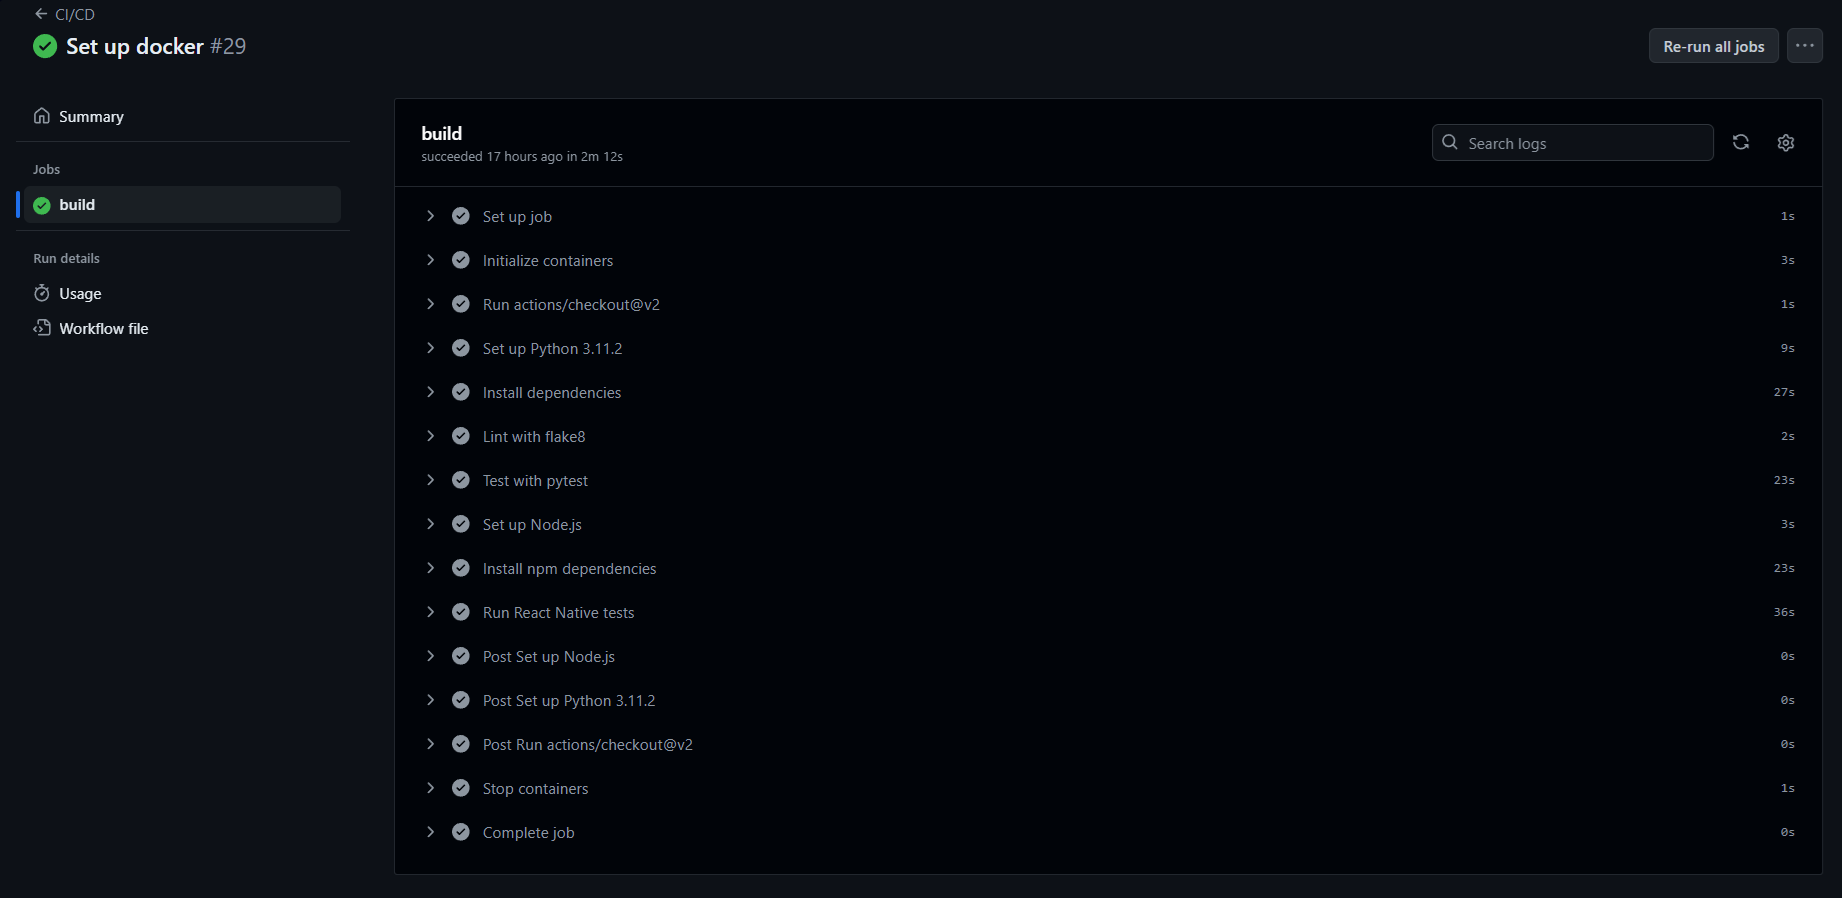
\includegraphics[width=1\linewidth]{LATEX/Appendices/Images/Pipeline_CI_CD/github_actions_CI_CD_pipeline.png}
    \caption{CI/CD Pipeline}
    \label{fig:CI/CD-Pipeline}
\end{figure}

\subsection{Continuous Deployment}

To be written soon...

\section{Software Evaluation Strategy}

As the testing phase concludes, the evaluation methods employed for the software merit a discussion. The infrastructure, including both the backend and the frontend, was thoroughly unit tested, adhering to Weak Robust Equivalence Class based testing and obtaining a 100\% coverage across key parameters such as lines, functions, statements, and branches. Additionally, the frontend's UI/UX was tested by collecting user feedback from fellow students. Moreover, the software was also evaluated through CI/CD processes, ensuring that updates were efficiently integrated and deployed without disruptions. Furthermore, the AI model was tested using a validation dataset, with the training loss maintained below 0.001 and the validation loss below 0.01. The delegation of job performance metrics evaluation to the backend, which remains unimplemented, resulted in a reduction of the AI model's intended scope. Rather than integrating these metrics at the time of contract translation into code — a task that was found to be unfeasible — the AI model's functionality was adjusted. This adjustment led to the AI model translating contractual clauses into nearly identical code, differing only in variables such as USDC addresses of employers and employees, starting and ending dates, contract token interfaces, and other case-specific details. This code's execution depends on the data related to an employee's job performance, which was intended to be passed to the deployed contract by the backend, revealing that there was no necessity for the AI model as this could have been accomplished through simple parsing. However, despite these unexpected outcomes, the primary objective to provide an infrastructure for employment management was met, obviating the need for a precise evaluation of the AI model and smart contracts' behaviour.

\section{Limitations and Scope for Future Development}

\subsection{Unimplemented Features}

An essential component of the project that was disregarded consisted of the backend's ability to monitor and upload job performance metrics into smart contracts after their deployment. This feature was necessary in order to completely automate blockchain-based employment interactions, and without it, the software remains incomplete. Unfortunately, it was not implemented because of the project's large scope and strict time constraints. Although this is certainly possible, the approach to addressing this challenge would be substantially difficult. To fill this void, one could explore the possibility of deploying an AI system capable of dynamically writing scripts that adapt to various employers' CRM systems. However, implementing such a model might be difficult. Alternatively, the system could evolve into a startup platform, where smart contracts are built with the aid of the software implemented. In this case, developers would manually create scripts to extract data from CRM systems and feed it into smart contracts for each specific case.  

\subsection{Reflective Analysis on Smart Contract Deployment Strategy}

At the outset of this project, there was a significant gap in understanding how smart contract technology operates. It was initially believed that a new smart contract was required for each work interaction. Since deploying smart contracts involves substantial costs, creating a separate smart contract for every employment interaction proved economically unviable. A more strategic approach, which was realised later, would involve developing a single general smart contract to manage all employment interactions while creating separate instances of it for various employment scenarios. This approach would significantly reduce the cost and complexity of smart contract deployment.

\section{Comparison of Achievements and Requirements}

In the following analysis, the initial requirements will be compared with the accomplished achievements. The comparison is categorised into functional and non-functional requirements:

\subsection{Functional Requirements}

\begin{itemize}
    \item \textbf{Contract Conversion:} Achieved. The platform successfully converts traditional employment contracts into smart contracts using a fine-tuned \texttt{GPT-3.5 Turbo} model.
    \item \textbf{AI Model Integration:} Achieved. The AI model has been successfully integrated with the backend, allowing for efficient processing of contracts.
    \item \textbf{User Authentication:} Achieved. Secure user account creation and management have been implemented.
    \item \textbf{User Engagement:} Achieved. A forum for user interactions on topics related to the application's scope has been developed.
    \item \textbf{Contract Management:} Achieved. Users can create, view, update, and delete their smart contracts in the application.
    \item \textbf{Performance Metrics:} Not achieved. Automating the monitoring and uploading of job performance metrics into smart contracts was deemed too complex and, due to time constraints, was not implemented. %ELABORATE HERE%
    \item \textbf{Salary Management:} Achieved. The system handles salary payments using \textit{USDC Coin}.
    \item \textbf{Notifications:} Achieved. Users receive notifications regarding contract updates, forum interactions, and other relevant events.
    \item \textbf{Mobile Application:} Achieved. A user-friendly interface for both \textit{iOS} and \textit{Android} platforms has been developed.
    \item \textbf{Custom Theming:} Achieved. The UI supports both dark and light modes.
    \item \textbf{Admin Panel:} Achieved. An admin panel for managing users, contracts, and system settings has been implemented.
    \item \textbf{Dispute Resolution:} Partially achieved. The platform provides mechanisms for resolving disputes, but it relies on job performance metrics, which are not implemented.
\end{itemize}

\subsection{Non-Functional Requirements}

\begin{itemize}
    \item \textbf{Scalability:} Partially achieved. Although the system architecture was designed to handle an increasing number of users and contracts efficiently, no adequate load testing was performed; no horizontal scaling was applied; and load balancers were not employed due to tight time constraints.
    \item \textbf{Security:} Achieved. The platform incorporates security measures to protect user data. This includes encryption for data in transit using HTTPS, secure user authentication methods, and secure storage of sensitive data on user devices through the \textit{expo-secure-storage} library. Additionally, the use of smart contracts ensures tamper-proof transactions due to the nature of the technology.
    \item \textbf{Reliability:} Not achieved. Although the platform seems reliable for now, there was no use of redundant systems, regular backups, or failover mechanisms. Unfortunately, time constraints prevented the implementation of these features.
    \item \textbf{Performance:} Achieved. The system provides quick response times for user interactions, contract processing, and AI model predictions. Thorough optimisation was applied during each sprint cycle to enhance the efficiency of all algorithms and code. Moreover, the software was designed to avoid heavy computations, with the exception of document translation into \textit{Solidity} code, which is executed on \textit{OpenAI's} servers.
    \item \textbf{Usability:} Achieved. The mobile application interface is intuitive, providing a positive user experience. User feedback was collected from peer students and incorporated during the development process to improve usability. In addition, the application supports both \textit{iOS} and \textit{Android} platforms.
    \item \textbf{Compliance:} Achieved. The platform complies with relevant regulations regarding employment contracts and data protection, such as GDPR. This was achieved through data anonymisation techniques, obtaining user consent for data usage, and ensuring that all data processing activities are compliant with legal standards.
    \item \textbf{Maintainability:} Partially achieved. While the codebase is modular, allowing for easy updates and maintenance, it sometimes lacks documentation. Even though the code is clean and self-explanatory, this could pose challenges for future developers who might need to understand the system.
    \item \textbf{Portability:} Achieved. Containerisation technique was applied with the aid of \textit{Docker} to package the application and its dependencies. This makes it easy to migrate the system to different cloud providers or on-premises servers if needed.
\end{itemize}

In conclusion, despite some unimplemented features and partial achievements, the project successfully met most of its initial requirements and objectives, laying a foundation for future development.

\section{Learning Outcomes}

This project has provided a solid learning experience, highlighting the importance of several industry best practices in software development. Some of the key lessons learned include:

\paragraph{Adherence to Test-Driven Development}

The primary lesson learned is the importance of adhering to Test-Driven Development (TDD). According to Boehm's curve, as software development proceeds, the cost of repairing bugs rises considerably. If TDD had been implemented from the outset, potential disruptions could have been mitigated early on. This might have even allowed for the correction of issues in the smart contract deployment strategy. Another significant learning point related to TDD adherence is the realisation that testing should not be left until the last moment, as it reveals critical bugs. More importantly, testing often proves more challenging than writing the original code, requiring three to five times more lines of code. Concluding, TDD allows for the clear definition of expected code behaviour, helping to maintain an architecture that is resistant to unnecessary future changes resulting from defects.

\paragraph{Continuous Integration and Continuous Deployment Practices}

Implementing a CI/CD pipeline is a must-have practice. It helps in maintaining a high standard of code quality through automated tests and, more importantly, in identifying issues as development progresses. 

\paragraph{Clear Definition of Requirements}

Another major takeaway from this project is that specific needs must be carefully defined before any development begins. Unclear requirements can lead to unnecessary project expansions, delays, and resource wastage.  In order to align the project's aims with the expected outcomes, all stakeholders must engage in thorough requirement gathering and validation.

\paragraph{Progress Tracking with Project Management Tools}

\texttt{Trello} and other project management tools have proven extremely effective for tracking progress and meeting deadlines. These tools provide clarity and accountability for the developers, assisting them in identifying bottlenecks early. Furthermore, an agile project management approach helps the development team react more readily to changes by encouraging regular feedback.

\paragraph{Iterative and Incremental Development}

Applying an iterative and incremental development approach is helpful. This technique enables scheduled releases with precise goals, allowing the team to test and refine the system by breaking it down into smaller components. Additionally, frequent demonstrations of progress help maintain stakeholder interest.

\paragraph{Documentation and Code Reviews}

The development process should involve detailed documentation and periodic code reviews. This is needed in order to ensure that the system is maintainable not only by the original developers, but also future team members. Additionally, regular code reviews also help preserve adherence to best software engineering principles, which in turn allows for easy knowledge sharing across the team.

\paragraph{User-Centred Design Focus}

Even though this was not incorporated in the project, it was later realised that maintaining a focus on user-centred design is crucial. Gathering feedback from users during the design phase allows the product to meet their expectations. Moreover, engaging users is essential for the project's financial success.

\paragraph{Risk Management and Mitigation Strategies}

Finally, proactive risk management should be an ongoing practice. Risk mitigation strategies should be developed for all potential risks identified at the outset and throughout the project's implementation. This involves regular risk assessment meetings and updating the risk matrix to address new challenges as they arise. 

\paragraph{Errors in Popular Frameworks}

Not all highly used frameworks are error-free. Given the complexities of modern software, even widely adopted frameworks contain errors and buggy code. For example, one issue encountered was related to React Native. During development, the UI was constantly returning the warning: "Animation Warning - Sending onAnimatedValueUpdate with no listeners registered." After extensive research, it was revealed that this well-known issue, related to the conditional rendering of screens in navigation, remains unresolved despite extensive documentation and community awareness \cite{GithubAnimatedViewWarning, StackOverFlowAnimatedViewWarning}.

\paragraph{Conclusion}

This project has demonstrated the significance of structured and disciplined software development processes. Each lesson learnt contributes to more efficient project management and execution in future software development projects.